\section{Problema de Valor de Contorno}


A solução de um problema regido por um modelo matemático depende de informações ligadas ao contexto em que tal problema ocorre.
Estas informações podem dizer a respeito das condições iniciais ou das condições de contorno. 
Condições iniciais caracterizam um \textbf{Problema de Valor Inicial (PVI)} e geralmente são relativas ao instante de tempo inicial do processo.
As condições de contorno por sua vez, caracterizam um \textbf{Problema de Valor de Contorno (PVC)} e  normalmente são dadas em função do limite espacial do processo em questão
\citep[p. 447]{boyce_diprima}.
Desta forma, enquanto os PVI geralmente relatam processos transientes, isto é, variantes no tempo, os PVC lidam com problemas em estado estacionário.

O PVI de um modelo de ordem $N$ é composto da equação do processo e do valor inicial da variável dependente e de suas derivadas, até a ordem $N-1$, como mostra a equação a seguir:

\begin{equation}
	\begin{cases}
		y'' + p(t)y' + q(t)y = f(t) \\
		y(t_0) = y_0 \\
		y'(t_0) = y_0'
	\end{cases}
\end{equation}

De forma análoga, o PVC é definido a partir da equação que modela o processo e suas condições nos pontos de contorno ou borda.

\begin{equation}
	\begin{cases}
		y''(x) + p(x)y'(x) + q(x)y(x) = f(x) \\
		y(x_i) = \alpha \\
		y'(x_f) = \beta
	\end{cases}
\end{equation}

Portanto, se as condições adicionais forem dadas em um único instante (ou ponto), tem-se o PVI do processo. Caso sejam dadas em dois ou mais pontos distintos, tem-se o PVC.

As condições de contorno usualmente podem ser classificadas como condições de Dirichlet ou de Neumann. 
As \textbf{condições de Dirichlet} são também conhecidas como \textbf{essenciais} e são estabelecidas sobre a variável dependente. Já as \textbf{condições de Neumann} são condições \textbf{naturais} e são impostas sobre as derivadas da variável dependente. A seguir são dados alguns exemplos.

\begin{equation}
	\begin{tabular}{l l}
		$y(x_k) = y_k $ 
		& Cond. Dirichlet \\
		$y(x_k) = 0$
		& Cond. Dirichlet Homogênea\  \\
		$y'(x_k) = y_k$
		& Cond. Neumann \\
		$y'(x_k) = 0$
		& Cond. Neumann Homogênea\  \\
	\end{tabular}
\end{equation}

A resolução analítica de PVC, ou mesmo de PVI, se torna impraticável à medida em que a complexidade do modelo, ou do contexto em que ele ocorre, aumenta.
Tal complexidade pode ocorrer, por exemplo, com a existência de coeficientes variáveis, regiões irregulares ou com condições de contorno inadequadas, existência de interfaces ou devido à grande quantidade de detalhes do problema
\citep[p. 410]{powers}.

Métodos numéricos apropriados podem ser utilizados na obtenção de uma solução aproximada para tais problemas. Neste trabalho serão abordados o \textbf{Método das Diferenças Finitas (MDF)} e o \textbf{Método dos Elementos Finitos (MEF)}.

A fim ilustrar o PVC, considere o seguinte exemplo  unidimensional, no qual um dado domínio $ \Omega $, contido no conjunto dos números reais, é limitado por uma borda $\Gamma$. 

\begin{equation}
	\begin{cases}
		\Omega = [a, b]  \\
		\Gamma = \{ a, b \} 
	\end{cases}
\end{equation}

Um PVC aplicado sobre a região $\Omega \cup \Gamma$ pode ser então dado pelo sistema a seguir. A parte $\Gamma_D$ da fronteira possui condição de contorno de Dirichlet, enquanto a parte $\Gamma_N$ possui condição de Neumann. Portanto, tem-se que $\Gamma = \Gamma_D \cup \Gamma_N$.

\begin{equation}
	\begin{cases}
		\begin{tabular}{l l}
			$y''(x) = p(x)y'(x) + q(x)y(x) + r(x)$ 
			& em $\Omega$  \\
			$y(a) = \alpha$ 
			& em $\Gamma_D$  \\
			$y'(b) = \beta$ 
			& em $\Gamma_N$
		\end{tabular}
	\end{cases}
\end{equation}

Resolver este problema consiste em encontrar a curva do modelo que satisfaz às condições de contorno. Um exemplo de curva solução é dado na figura \ref{fig:pvc}. É importante notar que, dependendo do modelo e das condições adicionais, um PVC pode possuir uma, nenhuma ou múltiplas soluções. Este comportamento se assemelha ao de equações algébricas lineares \citep[p. 448]{boyce_diprima}. Conforme o princío de Hadamard, o problema é dito \textbf{bem posto} se tiver solução única, caso contrário, será dito \textbf{mal posto}.

\begin{figure}[ht!]
\centering
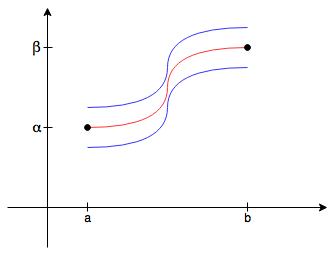
\includegraphics[scale=0.5]{figuras/pvc.png}
\caption{PVC: Encontrar a curva solução entre os pontos $ (a, \alpha) $ e $ (b, \beta) $}
\label{fig:pvc}
\end{figure}

